%! Author = jonathan
%! Date = 5/26/25
\chapter{Introduction}\label{ch:introduction}
State-of-the-art large language models (LLMs), including DeepSeek-v3~\cite{deepep}, LLama4~\cite{llama4},
DBRX~\cite{dbrx} and Snowflake Arctic~\cite{arctic}, have adopted the Mixture-of-Experts (MoE)
~\cite{DBLP:conf/iclr/ShazeerMMDLHD17}
architecture for its computational efficiency~\cite{pmlr-v162-rajbhandari22a} and reliable
performance across language modeling tasks~\cite{deepep, llama4, jiang2024mixtralexperts}.
\begin{figure}[!ht]
    \centering
    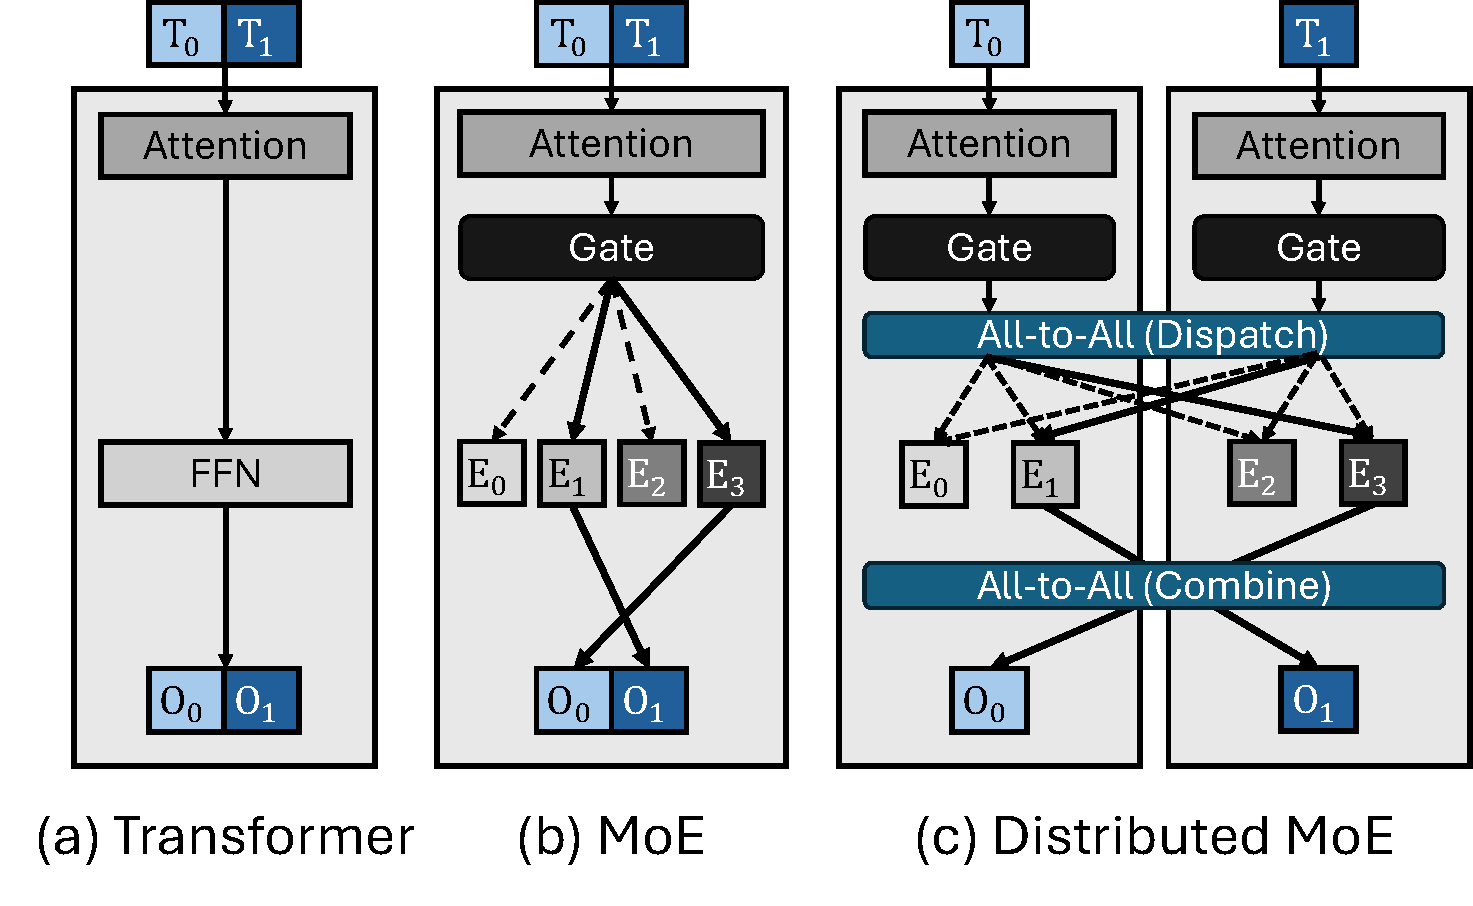
\includegraphics[width=0.55\textwidth, keepaspectratio]{figures/fig-bg-moe}
    \caption{Transformer blocks (a) without MoE, (b) with MoE, and (c) with distributed MoE and expert parallelism.
        \texttt{T}, \texttt{E}, and \texttt{O} represent input tokens, experts, and output activations, respectively.}
    \label{fig:bg:moe}
\end{figure}

Depicted in Figure~\ref{fig:bg:moe}(a), the conventional Transformer block consists of
a self-attention module followed by a feed-forward network (FFN)~\cite{NIPS2017_3f5ee243}.
In contrast, MoE architectures replace this single FFN with identically sized FFNs,
otherwise known as experts, (Figure~\ref{fig:bg:moe}(b)).
A trainable neural network, known as a gate function, sparsely activates these experts by
dynamically routing input tokens to selected experts at runtime.
This increase in model parameters (more FFNs) improves model quality without a
\textit{corresponding increase in computational cost}.
\section{Computational Cost Equivalence}\label{sec:comoutational-cost-equivalence}
The preceding claim seems counterintuitive because \emph{shouldn't the increase in the number of experts
yield a proportional increase in the model's computational operations?}
The answer is no, due to how tokens are \emph{distributed} across experts in comparison to the singular FFN.
For example, consider a token matrix $T$ as defined below where $S$ is the sequence length and $H$
the embedding dimension.
\[
    T \in \mathbb{R}^{S \times H}
\]
The typical FFN operator, defined below,
\begin{equation}\label{eq:ffn}
\textrm{FFN}(x) = W_2 \cdot \phi(x W_1 + b_1) + b_2
\end{equation}
comprises two linear transformations on learnable weight matrices
$W_1\in \mathbb{R}^{H \times P}$, $W_2 \in \mathbb{R}^{P \times H}$ each followed by additions with bias terms
$b_1 \in \mathbb{R}^{1 \times P}$, $b_2 \in \mathbb{R}^{1 \times H}$ and separated by a
nonlinear activation $\phi$ (e.g., GELU~\cite{hendrycks2023gaussianerrorlinearunits} or
ReLU~\cite{10.5555/3104322.3104425}).
Here dimension $P$ is an intermediate projection for the FFN\@, typically $P = 4\cdot H$~\cite{NEURIPS2024_9f2b171f}.
If we define $\mathcal{F}_{FFN}$ as the \textbf{F}loating \textbf{P}oint \textbf{OP}erations (FLOPs)
needed to compute a forward pass of the FFN, then using Equation~\ref{eq:ffn} we have the resulting expression.
\begin{equation}\label{eq:flopsffn}
\mathcal{F}_{FFN} = \mathcal{F}_{L_0} + \mathcal{F}_{L_1}
\end{equation}
where $\mathcal{F}_{L_i}$ is the FLOPs cost for computing linear transformation $i$.
These linear transformations are \textbf{GE}neral \textbf{M}atrix \textbf{M}ultiplications (GEMMs).
We know that multiplying two matrices of sizes $(M, K)$ and $(K, N)$ demands $2MNK$ FLOPs,
therefore we can expand Equation~\ref{eq:flopsffn} as
\begin{equation}\label{eq:flopsffn2}
\mathcal{F}_{FFN} = 2SHP + 2SHP = 4SHP
\end{equation}

An MoE model differs from the dense transformer by \emph{restricting} the number of
tokens~\cite{DBLP:conf/iclr/LepikhinLXCFHKS21, MLSYS2023_5a54f793} routed to an FFN
(interchangeably called expert).
Specifically, for a model with $N_e$ experts, each expert has a fixed capacity for tokens $S_e$ defined as follows
\begin{equation}\label{eq:capacity}
S_e = \frac{S}{N_e}
\end{equation}
With the above, we can compute $\mathcal{F}_{MoE}$.
Intuitively, this quantity would be the aggregate of $\mathcal{F}_{{FFN}_j}$ where $j \in \{0, \cdots, N_e - 1\}$.
\begin{equation}\label{eq:flopsmoe}
\mathcal{F}_{MoE} = \sum\limits_{j = 0}^{N_e - 1}\mathcal{F}_{{FFN}_j}
\end{equation}
Observe that $\mathcal{F}_{{FFN}_j}$ is derivable from Equation~\ref{eq:flopsffn}
by replacing $S$ with $S_e$.
Applying this observation and evaluating~\ref{eq:flopsmoe} gives the below result
\begin{equation}\label{eq:flopsmoe2}
\mathcal{F}_{MoE} = N_e \cdot 4S_{e}HP
\end{equation}
Substituting with~\ref{eq:capacity}, yields the below which proves that the computational cost is equivalent
between the MoE and dense transformer models!
\begin{equation}\label{eq:equivalence}
\mathcal{F}_{MoE} = 4SHP = \mathcal{F}_{FFN}
\end{equation}
This relationship presents empirically as uniform latency when $N_e$
increases but only till a certain threshold.
Exceeding this limit causes the latency to increase proportionally;
existing work gives no explanation for this phenomenon, but we
hypothesize GPU L1/L2 cache thrashing to be the culprit.

\section{Communication Overheads in Distributed MoE}\label{sec:communication-overheads-in-distributed-moe}
\begin{figure}[!ht]
    \centering
    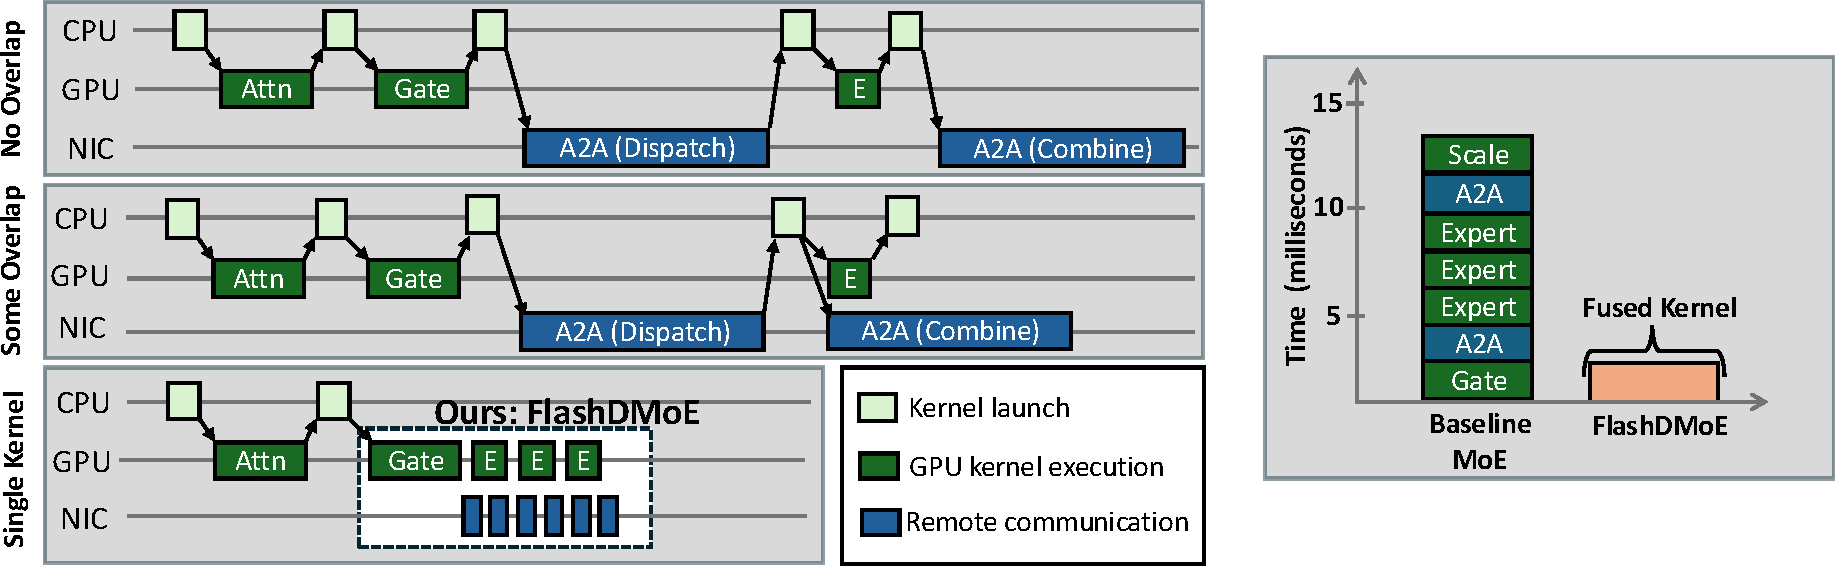
\includegraphics[width=0.98\textwidth, keepaspectratio]{figures/intro-fig}
    \caption{Comparing \sysname with state-of-the-art techniques that either do not overlap communication and
    computation (left, top) or do some overlap (left, middle). \sysname is a persistent kernel that fuses all
    computation and communication of the MoE operator (left, bottom). \sysname implements
    device-initiated computation (gate, expert FFN, scale) and communication tasks (right).}
    \label{fig:intro}
\end{figure}
As MoE model sizes grow, GPU memory constraints prevent hosting all experts on a single device.
The standard practice is to distribute experts across multiple GPUs using expert parallelism (EP),
which requires the gate function to route tokens via \alltoall communication
~\cite{deepep, arctic, dbrx, 10.1145/3577193.3593704}.
Overall, each MoE layer executes two \alltoall operations during inference,
introducing significant communication overhead. \alltoall communication is challenging to optimize on GPU networks
and is highly sensitive to straggler delays---a phenomenon where a single \emph{straggler} GPU delays
all others from making progress.
In practice, these communication operations can account for up to 40\% of the total runtime during inference or
training~\cite{10.1145/3603269.3604869, MLSYS2024_339caf45}.
\section{Kernel Launch Overheads in Distributed MoE}\label{sec:kernel-launch-overheads-in-distributed-moe}
\begin{table}[!ht]
    \centering
    \small
    \setlength{\tabcolsep}{8pt}
    \renewcommand{\arraystretch}{0.9}
    \begin{tabular}{@{}lc@{}}
        \toprule
        \textbf{Works} & \textbf{Launched GPU Ops} \\ \midrule
        \sysname & 1 \\
        COMET~\cite{comet} & 33 \\
        Megatron-LM CUTLASS~\cite{megatron, 10.1145/3458817.3476209} & 85 \\
        Megatron-LM TE~\cite{megatron, 10.1145/3458817.3476209} & 261 \\
        Megatron-LM + DeepEP~\cite{deepep} & 432 \\
        DeepSpeedMoE~\cite{pmlr-v162-rajbhandari22a} & 550 \\
        \bottomrule
    \end{tabular}
    \caption{\textbf{Kernel Fusion Comparison.}
    Our method is the first to fully fuse the DMoE layer into a single GPU kernel.
    We report GPU operations from detailed profiling with Nsight Systems.}
    \label{tab:gpuOps}
\end{table}
To mitigate these communication bottlenecks,
recent work pipelines computation with communication tasks
(Figure~\ref{fig:intro}, middle left).
However, the effectiveness of these solutions is limited by the overhead of
launching many kernels from the CPU\@.
Specifically, MoE layers interleave multiple computation kernels
(such as gate and expert computations) and communication operations,
forcing the CPU to launch many GPU kernels per forward pass
(see Table~\ref{tab:gpuOps}).
Frequent kernel launches negatively affect performance by:
(1) creating non-deterministic kernel start times across GPUs, exacerbating straggler issues;
(2) introducing unnecessary synchronization points,
causing GPUs to wait on peers or the CPU before proceeding;
and (3) incurring repeated global memory round trips at kernel boundaries.
Although CUDA graphs~\cite{cuda_graphs_nvidia_blog} can partially mitigate the
first issue in static workloads,
they are incompatible with MoE's dynamic expert routing patterns.
Addressing the remaining issues requires novel solutions,
which we provide in this work through complete kernel fusion and
asynchronous device-initiated communication.
\section{This work's Contributions: DMoE in a single kernel}\label{sec:contributions:-moe-operator-in-a-single-kernel}
To overcome these fundamental inefficiencies in state-of-the-art MoE models,
we develop \sysname, a novel MoE architecture that integrates all computation
and communication tasks into a single persistent GPU kernel, namely
a kernel that remains active for the entirety of the MoE operator
(Figure~\ref{fig:intro} bottom left).
Instead of multiple kernel launches coordinated by the CPU,
\sysname requires launching only one kernel,
significantly reducing the involvement of the CPU in the MoE operator.
Within the fused kernel, \sysname implements a concurrent-programming
model to achieve fine-grained parallelization
of computation and communication tasks of the MoE operator.
This design enables \sysname to efficiently utilize GPU resources by reducing idle time.
\subsection{Warp Specialization and Tile Parallelism.}\label{subsec:wstp}
\begin{figure}[!ht]
    \centering
    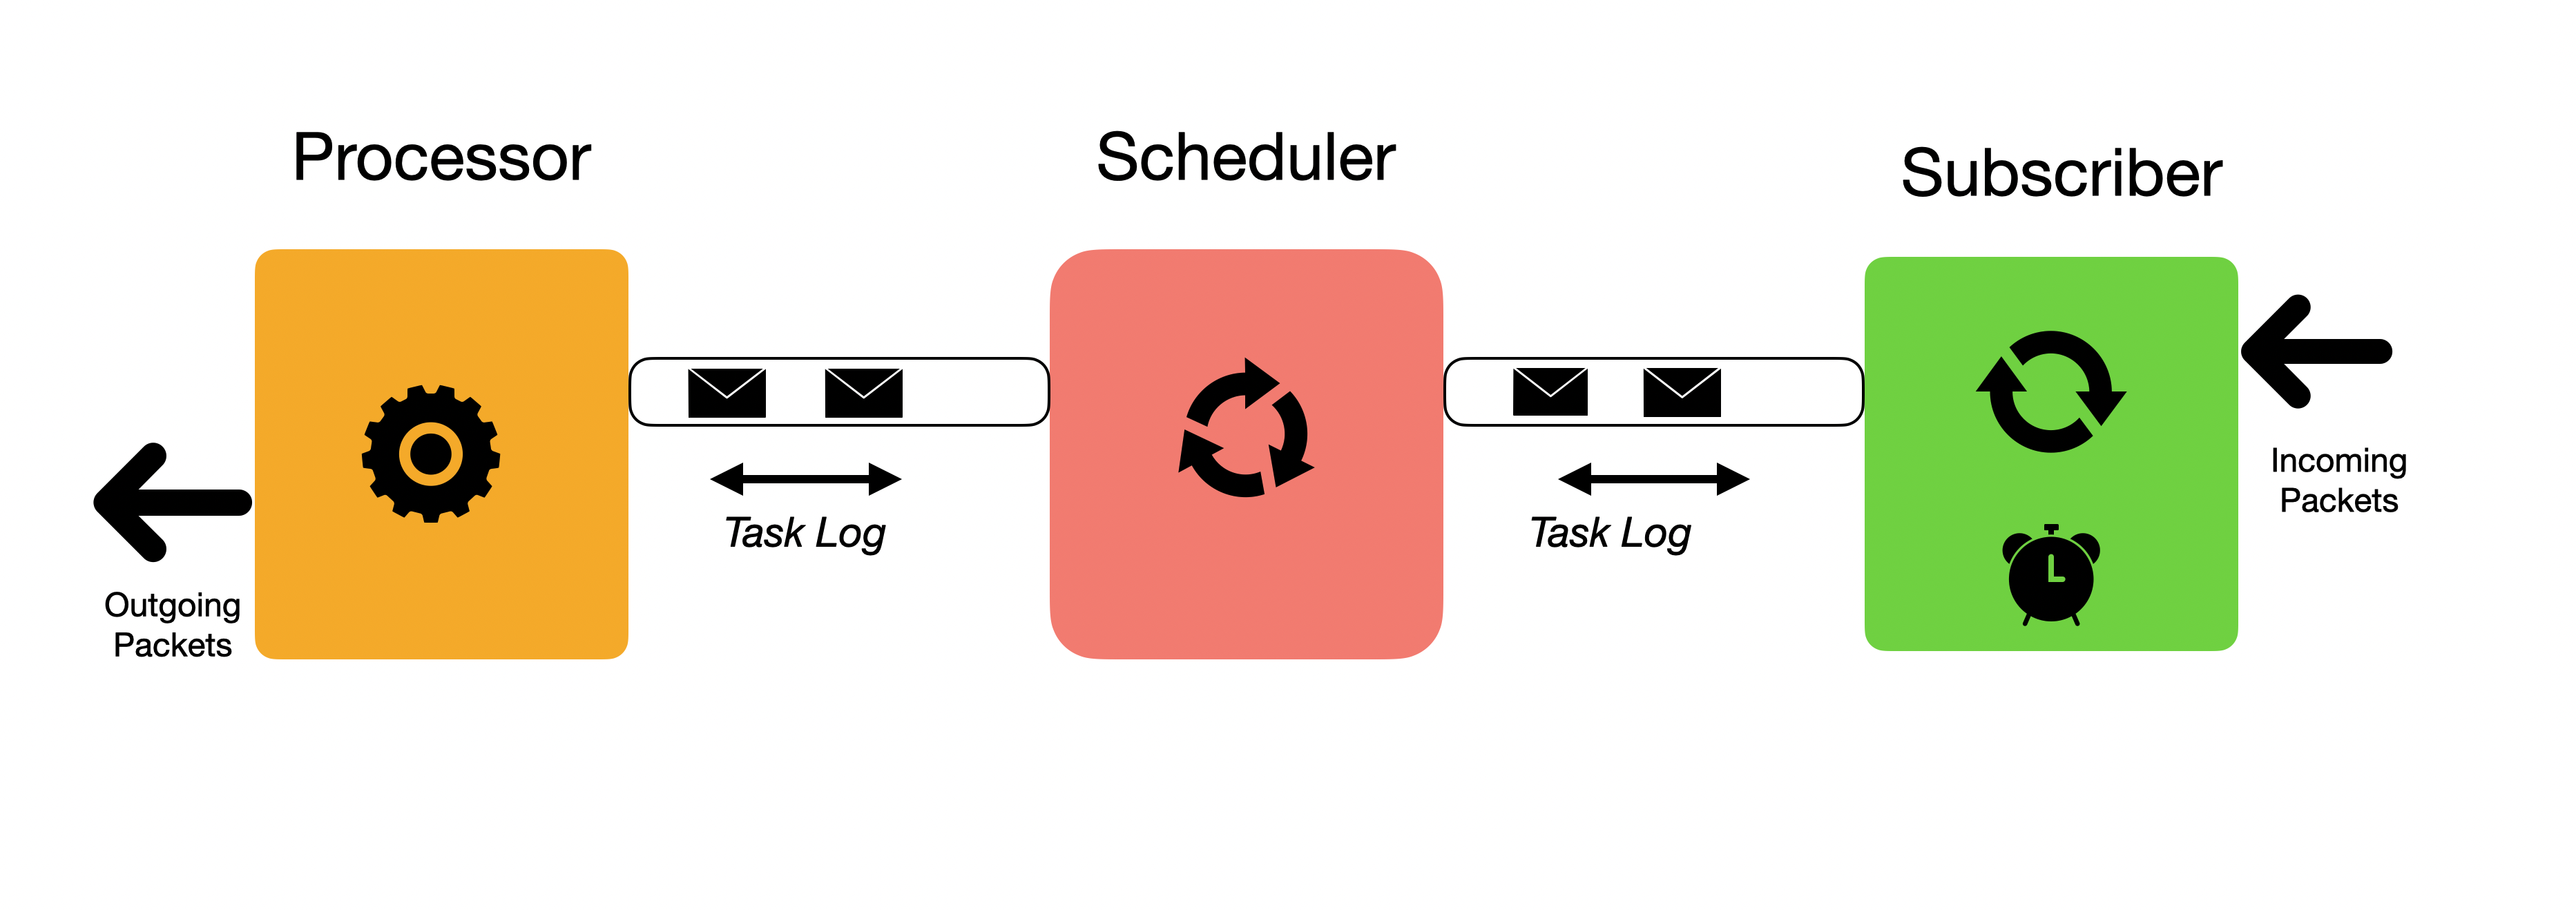
\includegraphics[width=0.98\textwidth, keepaspectratio]{figures/flash_actors}
    \caption{\sysname Actors. The \textcolor{LimeGreen}{Subscriber} observes received remote \emph{packets}
    (blob of tiles), decodes them into \emph{tasks} and notifies the scheduler of the enqueued tasks.
    We assign three CUDA warps to this role.
    The \textcolor{Salmon}{Scheduler} maintains a \emph{ready queue} of \textcolor{Orange}{Processors}
    from which it schedules tasks. The \textcolor{Yellow}{Processors} performs the operation encoded in its task
    descriptor and eagerly communicates its output, if necessary.}
    \label{fig:flash_actors}
\end{figure}
\sysname implements \emph{tile-level parallelism},
meaning it partitions input token matrices into smaller,
independent units called \emph{tiles},
which are processed concurrently by GPU thread warps.
These warps specialize as \emph{processors}
since they process input to compute the gate function and expert FFNs.
A handful of warps perform specialized administrative tasks of
(1) scheduling computational tasks by mapping them to warps (\emph{scheduler}), and
(2) communicating with other GPUs (\emph{subscriber}).
This design allows \sysname to dynamically assign tasks to GPU warps based
on warp availability and the current workload,
ensuring that no warp remains idle while useful work can be done.
\sysname selects tile dimensions to maximize GPU arithmetic intensity and
minimize register pressure.
\subsection{Asynchronous and payload-efficient communication.}\label{subsec:asynchronous-and-payload-efficient-communication.}
\begin{figure}[!ht]
    \centering
    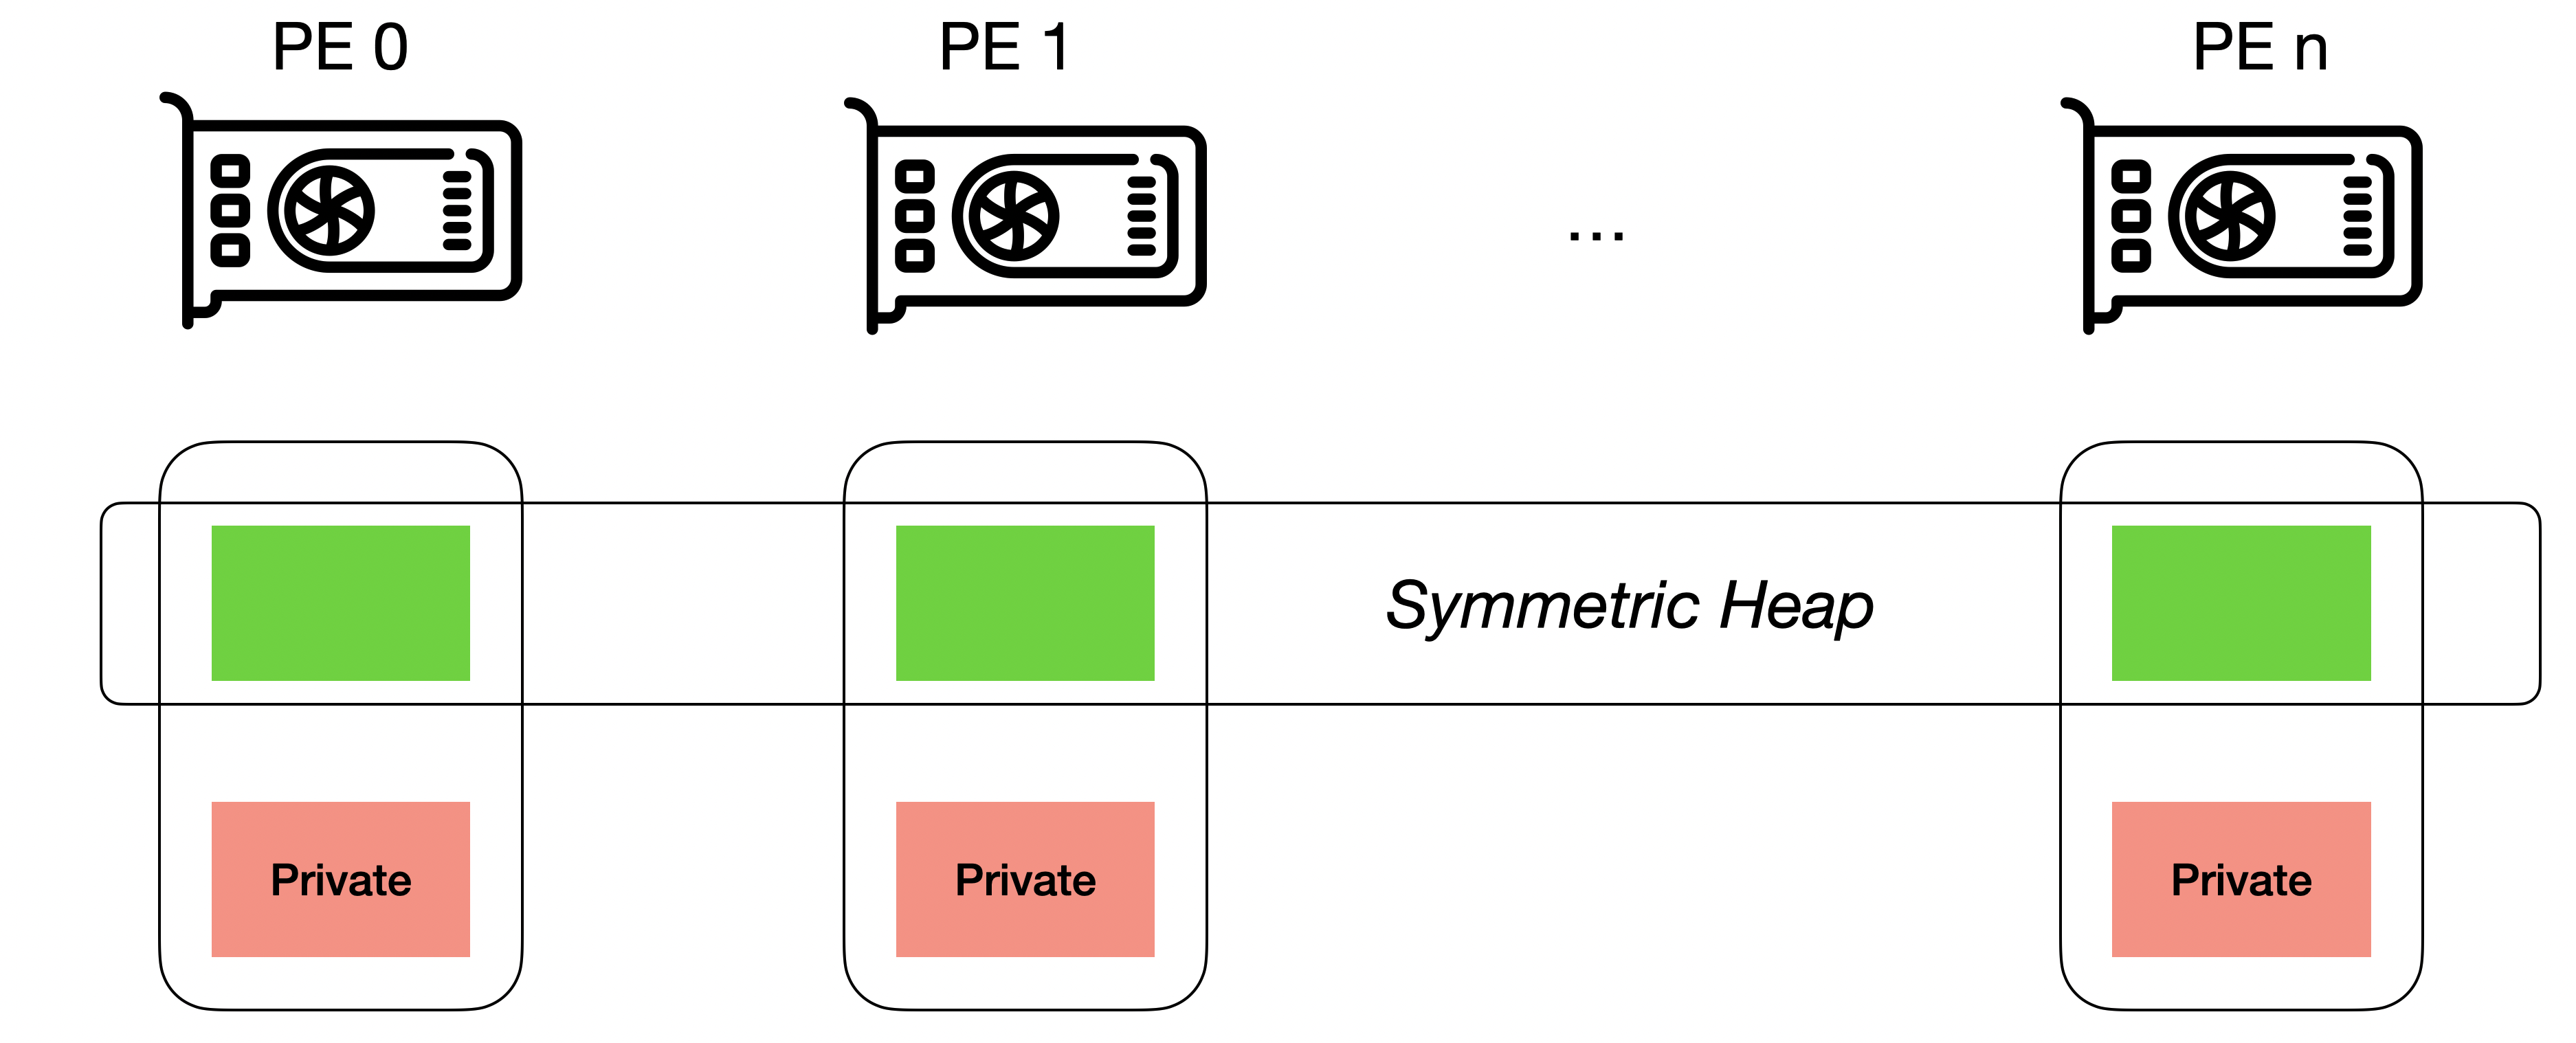
\includegraphics[width=0.98\textwidth, keepaspectratio]{figures/pgas}
    \caption{Depiction of a Partitioned Global Adress Space (PGAS)~\cite{10.1145/1278177.1278183}
        across a \textit{team} of \textbf{P}rocessing \textbf{E}lements (PEs). The symmetric heap is an
    unifromly sized memroy region resident on each PE and accessible by every other PE via one-sided
    \textbf{D}irect \textbf{M}emory \textbf{A}ccess (DMA) or \textbf{R}emote DMA (RDMA) operations.}
    \label{fig:pgas}
\end{figure}
By redesigning the MoE operator from the ground up,
\sysname resolves fundamental inefficiencies inherent
in the conventional MoE execution pipeline.
One inefficiency is due to workload imbalance across GPUs due to
skewed popularity of experts.
Existing implementations~\cite{pmlr-v162-rajbhandari22a} indiscriminately perform \alltoall communications,
transferring null values to GPUs that host unpopular experts,
resulting in wasted communication bandwidth and unnecessary computations on null matrices.
\sysname introduces \emph{payload-efficient} communication
by sending tokens only to GPUs with actively selected experts,
thereby conserving both communication and computational resources.
\subsection{Technical Challenges}\label{subsec:technical-challenges}
Realizing the single-kernel design of \sysname required solving several
technical challenges.
\sysname's design is a radical departure from
traditional synchronous \alltoall collectives,
where GPUs remain idle until the slowest GPU completes its communication.
Instead, \sysname establishes a global address space via NVSHMEM~\cite{nvshm} across all GPUs to
achieve asynchronous communication between GPUs while allowing them to
continue performing useful computation tasks.
To implement device-initiated computation primitives,
\sysname develops custom high-performance GEMM operations for the MoE operator in
CUTLASS~\cite{Thakkar_CUTLASS_2023}.
\subsection{Research Papers}\label{subsec:research-papers}
This thesis comprises a first-author publication~\cite{10.1145/3725536.3725539} at ACM SIGMETRICS'24 and another first-author
submission in review at NeurIPS \('25\).

